\documentclass[12pt,a4paper]{scrartcl}

%\usepackage{german}
\usepackage[utf8]{inputenc}
\usepackage{graphicx}

\usepackage{url}
%\urldef{\urlTcpdump}{\url}{http://www.tcpdump.org/}

\usepackage{hyperref}
\hypersetup{colorlinks=false,pdfborder={0 0 0}}

\usepackage{biblatex}
%\usepackage[style=alphabetic]{biblatex}
\ExecuteBibliographyOptions{hyperref=true,language=ngerman,backref=true}
\addbibresource{bibliography.bib}

%\usepackage{lineno}
%\linenumbers

% Shorten the usage of german quotation marks.
\newcommand{\gq}[1]{
	\glqq #1\grqq
}

% Inline comment.
\newcommand{\comment}[2]{#2}
\newcommand{\todo}[2]{#2}

% Vertical space after paragraph.
\newcommand{\s}{\vspace{0.5em}}

% Little table for most important software info.
\newcommand{\infotable}[4]{
	\begin{tabular}{p{2.5cm}l}
		Website: & \url{#1} \\
		Language: & #2 \\
		Last commit: & #3 \\
		Commits: & #4 \\
	\end{tabular}
	\s
}

% Emphasize a criterion.
\newcommand{\crit}[2]{\textbf{#1} (#2)}

% Aliases for yes and no in comparison overview table.
\newcommand{\y}{\checkmark}
\newcommand{\n}{$\times$}

% Easy reference to section name and page.
\newcommand{\textref}[1]{"\nameref{#1}" on page \pageref{#1}}

% Palatino
\renewcommand*\rmdefault{ppl}
%\renewcommand{\baselinestretch}{1.125}
\renewcommand{\baselinestretch}{1.1875}

% Times
%\usepackage{times}

% Iwona
%\renewcommand*\rmdefault{iwona}



\begin{document}

	\title{Møil: A web-based administration tool for mail servers backed by relational databases}
	\author{Henning Müller $<$\href{mailto:henning@orgizm.net}{henning@orgizm.net}$>$}
	\date{}

	\maketitle


	\section*{Abstract}
		This document compares existing administration user interface solutions
		for mail servers backed by relational databases and introduces yet
		another one, which is called Møil and is written in Ruby utilizing the
		Ruby on Rails\footnote{\url{http://rubyonrails.org}} framework. It
		brings the handy possibility of managing the database schema with
		migrations, a lot of beautiful, responsive CRUD and some other nice
		features (see page \pageref{moeil-features}). The code is available from
		GitHub\footnote{\url{https://github.com/nning/moeil}} licensed under
		AGPLv3 \cite{agpl}.

	\section*{Introduction}
		% Reasons for database-backing

		For mail system setups (meaning one or more servers running Mail
		Submission, Delivery and Transfer Agent software and providing a
		Message Store for users \cite{mail-architecture}), storing data about
		which domains and E-Mail addresses the system is responsible for
		(further called meta data) in relational databases (as opposed to plain
		files for example) is beneficial for several reasons.

		%	Horizontal scalability

		In bigger setups, it offers the possibility for scaling to more than
		one node (horizontal scalability) to cope with high mail and user
		loads: Several servers handling incoming mail or users reading their
		mail act as readers on one or more database servers. The performance of
		the frequent lookups of domains, mailboxes and aliases (forwardings)
		for receiving mail or user logins can be increased. (The actual
		accommodation of E-Mails -- another big problem with horizontal scaling
		-- can not be considered here.)

		%	API (e.g. for accounting)

		Database Management Systems (DBMS) for relational databases usually
		provide a query interface with the Structured Query Language (SQL)
		\cite{sql} for editing the data sets. It is widely supported by
		programming languages and equally widely spoken among programmers, which
		makes it valuable for integration of several services dealing with this
		mail system meta data. For example this can be used to integrate
		accounting solutions for charging purposes into mail systems.

		%	Structural clarity for administrators

		Another reason for the usage of relational databases as mail system
		meta data storage is the increased structural clarity for
		administrators. In a typical SMTP server setup (without a relational
		database), the relevant data for domains, mailboxes and aliases is
		distributed to several files. The existence of a domain is stated
		independently of the existence of a mailbox of the same domain or the
		password of this mailbox. The data is not interconnected; a mailbox
		address is usually not checked against the list of domains for
		consistency. For bigger mail system setups, this meta data
		configuration inevitably gets unmaintainable.

	\section*{Evaluation of existing software}
		% Overview and inspiration

		Although an extensive evaluation of the existing administration user
		interfaces did not happen before implementing a custom solution, some
		of the programs were still sighted and some of the following criteria
		was still considered. This more systematical and detailed analysis
		shall gain an overview and provide inspiration for the development of
		Møil.

		\subsection*{Criteria}
			% Data model
			%	Structure (postfix.admin compatible?)
			%	Maintainability of schema
			%	Security (e.g. password hashing)
			% Responsiveness
			%	Terminal
			%	Desktop web browsers
			%	Mobile devices
			% Usability
			% Scalability (for user exposed functionality)
			% Features
			%	Basic domain, mailbox and alias management
			%	Password change for end users
			%	Privilege model
			%	Others
			%		Audit trail
			%		Vacation
			%		Spam frontend
			%		Sieve
			%		Webmail integration
			% Programming language
			% Containability (e.g. independence of Message Store file system)
			% Database independence
			% Security, robustness, tests

		\subsection*{The contestants}
			\subsubsection*{modoboa}
				\infotable{http://modoboa.org}{Python}

			\subsubsection*{postfix.admin}
				\infotable{http://postfixadmin.sourceforge.net}{PHP}

			\subsubsection*{ratuus}
				\infotable{http://www.ratuus.org}{PHP}

			\subsubsection*{VBox.Adm}
				\infotable{http://www.vboxadm.net}{Perl}

			\subsubsection*{ViMbAdmin}
				\infotable{http://www.vimbadmin.net}{PHP}

	\section*{Møil}
		% Rails
		% Causes for a new solution
		%	Data model, migrations
		%	CLI
		%	Password hash generation for compatibility to older solution
		%	Other features

		\label{moeil-features}
		\subsection*{Features}

		\subsection*{Architecture}
			% Modules

		\subsection*{Data model}
			% Data model
			%	Structure / ERD
			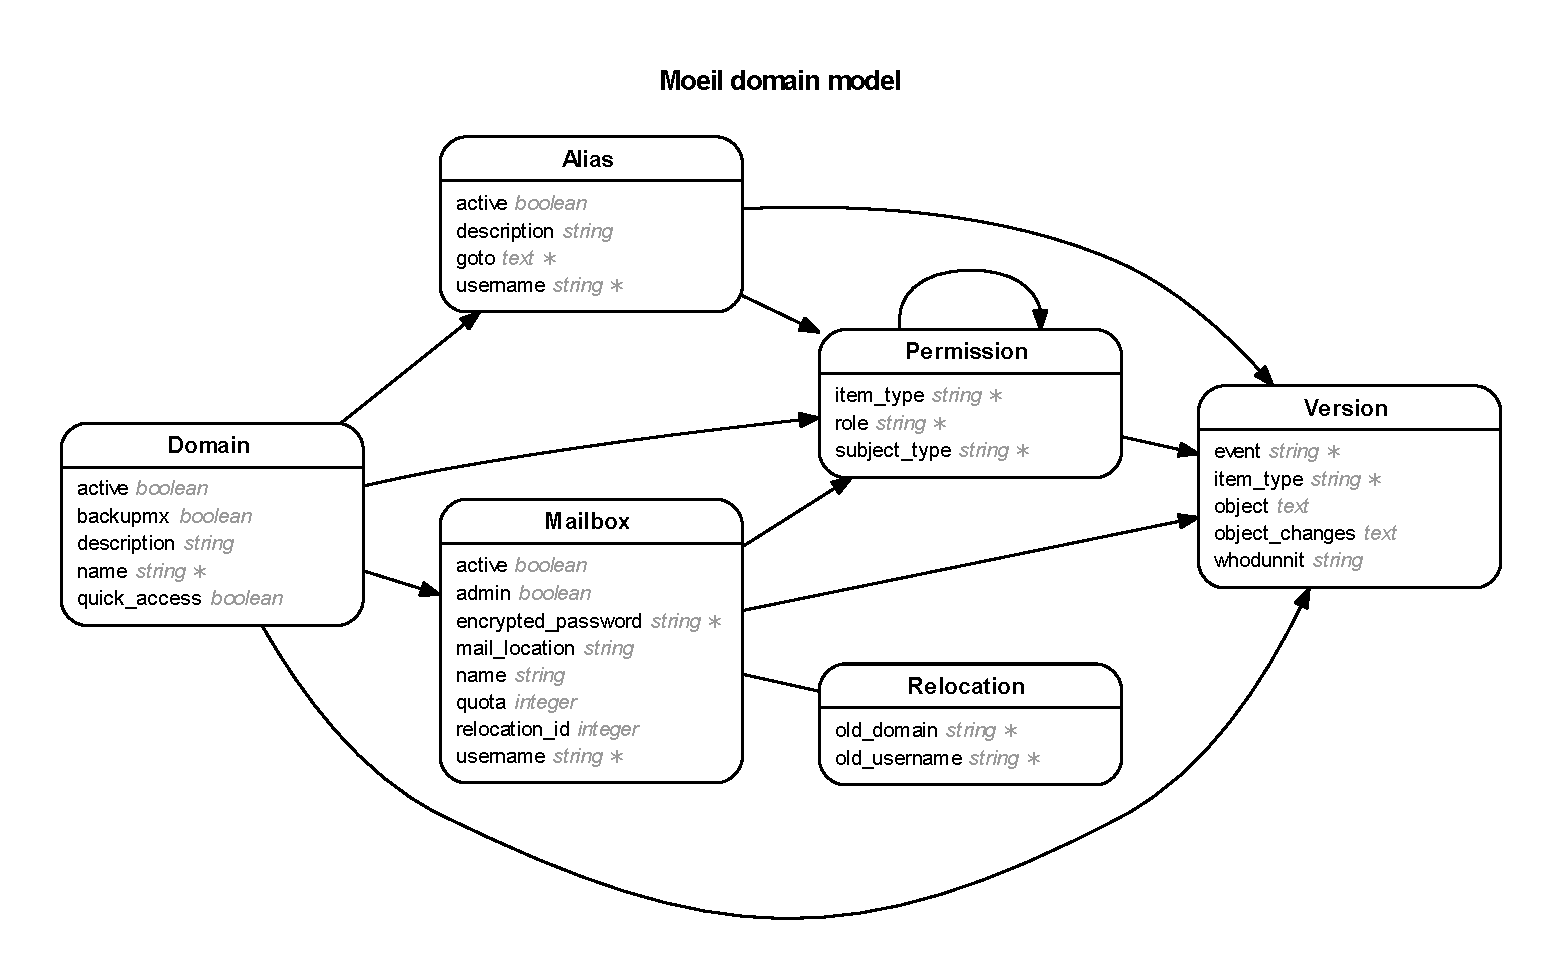
\includegraphics[width=\textwidth]{images/erd.pdf}
			%	Migrations
			%	sha512-crypt

		\subsection*{Setup}
			% Relevant configs for postfix and dovecot
			% Setup of rails app
			% Links to README on GitHub

	\printbibliography

\end{document}
